\documentclass[a4paper]{article}
\usepackage{listings}
\usepackage{qtree}
\usepackage{xcolor}
\usepackage{forest}
\usepackage{multicol}
\setlength{\columnsep}{3cm}
\usepackage{parskip}
\usepackage{changepage}
\usepackage[T1]{fontenc}
\usepackage{amsmath}
\usepackage{hyperref}
\usepackage{listings}
\usepackage{amsthm}
\usepackage{amssymb}
\usepackage{float}
\usepackage[utf8]{inputenc}
\usepackage{graphicx}
\usepackage[italian]{babel}
\usepackage{thmtools}
\newcommand{\channel}{\textit{channel }}
\newcommand{\pacchetto}{\textit{pacchetto }}

\begin{document}

\author{Lorenzo Dentis, lorenzo.dentis@edu.unito.it}
\title{Esercizi con Uppaal}
\maketitle
%http://ppedreiras.av.it.pt/resources/empse0809/slides/TheUppaalModelChecker-Julian.pdf
\section{Modello A}
Stop and wait e canale perfetto.\\ 
Si assume che il canale sia perfetto, e quindi nè il messaggio, nè l’ack possono essere persi. 
Il tempo di trasmissione sul link è variabile all’interno di un intervallo limitato (costanti minTransmissionTime e maxTransmissionTime ), con una differenza $\leq \frac{1}{10}$ tempo di trasmissione. 

Si definiscano e provino le proprietà di corretto funzionamento del protocollo, inparticolare si provi qual è il tempo minimo e massimo che intercorre dalla spedizione di un messaggio alla ricezione del suo ack.
\subsection{Mittente}
\begin{center}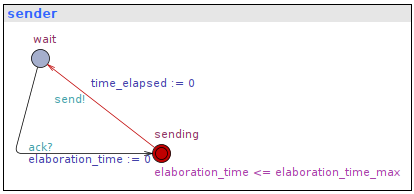
\includegraphics[width=0.8\textwidth]{1_sender.png}\end{center}
Il mittente prepara un messaggio,lo invia un e rimane in attesa di ricevere un Acknowledge, per poterlo inviare si sincronizza sul \channel send (tramite \texttt{send!}) e per riceverlo si sincronizza sul \channel ack (tramite \texttt{ack?}).
Quando un messaggio viene invato viene avviato un timer, \textit{time\_elapsed}, che sarà utile in fase di analisi per stabilire quanto tempo è passato dall'invio del messaggio alla ricezione dell'ack.
\subsection{Destinatario}
\begin{center}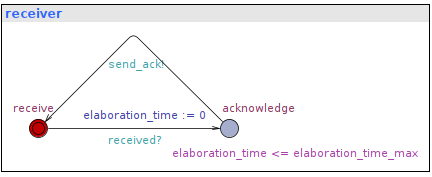
\includegraphics[width=0.8\textwidth]{1_receiver.png}\end{center}
Il destinatario può solo attendere la sincronizzazione sul \channel received, quando il canale gli fornisce un messaggio il Destinatario risponde con un Acknowledge che viene inviato sul canale sincronizzandosi sul \channel send\_ack.
\subsection{Canale}
Il canale presentato è un canale perfetto, quindi riceve un messaggio o un ack e lo consegna senza possibilità di perderlo.
Il canale è half-duplex, quindi permette la trasmissione non simultanea sia da mittente a destinatario che viceversa.\\
\begin{center}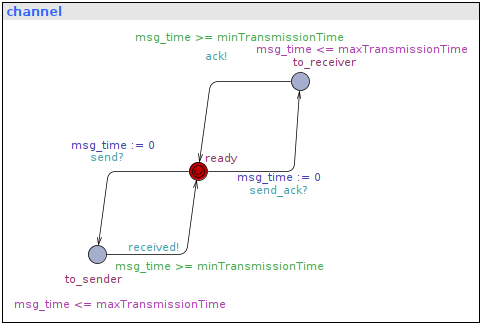
\includegraphics[width=1\textwidth]{channel_safe.png}\end{center}
Il canale quando non sta trasmettendo un messaggio si trova nello stato \textit{ready}, se il messaggio proviene dal mittente il canale si sincronizza sul \channel send e si sposta nello stato \texttt{to\_sender}, da questo stato esce solo dopo \textit{minTransmissionTime} e prima di \textit{maxTransmissionTime}, per rappresentare il tempo di trasmissione varibile del canale.
Per consegnare il messaggio si sincronizza con il Destinatario sul \channel received.\\
discorso diametralmente opposto vare per l'Acknowledge, il canale si sincroniza con il Destinatario sul \channel send\_ack, e consegna l'ack dopo un intervallo di tempo sincronizzandosi con il Mittente sul \channel ack.
In ultimo è presente un timer che viene resettato sull'arco di "presa in carico" di un \pacchetto, questo timer può esssere utilizzato per verificare il tempo necessario alla trasmissione di un singolo \pacchetto.
\subsection{Analisi}
\begin{itemize}
	\item \textit{A[] not deadlock}
		Il sistema non presenta stati di deadlock.
	\item \textit{A[] sender.prepare imply ((time\_elapsed >= 2 * minTransmissionTime \&\& time\_elapsed <= 2 * maxTransmissionTime) || time\_elapsed == 0)}
		Quando il mittente si trova nello stato \textit{prepare} il tempo trascorso può avere solo due valori: 0 se non è ancora stato inviato nessun messaggio oppure un valore compreso tra 2* tempo di trasmissione minimo e 2* tempo di trasmissione massimo. Infatti perchè il Mittente consideri il messaggio ricevuto e torni nello stato prepare deve aver ricevuto un ack, il tempo per ricevere un ack è il doppio del tempo necessario a trasmettere un \pacchetto
	\item \textit{sender.sending --> sender.prepare}
		Questa condizione è verificata in quanto se invio un messaggio ottengo un ack
	\item \textit{sender.sending --> receiver.acknowledge}
		Questa condizione è verificata in quanto se invio un messaggio il Destinatario lo riceve
	\item \textit{channel.to\_sender --> channel.to\_receiver}
		Questa verifica è effettuata per assicurarsi che in questo sistema quando il canale prende in carico un messaggio lo consegna sempre al Destinatario
	\item \textit{channel.ready --> (channel.ready \&\& msg\_time >= minTransmissionTime \&\& msg\_time <= maxTransmissionTime)}
		Questa condizione è verificata perchè se parto da uno stato in cui il canale e pronto a trasmettere tornerò dopo qualsiasi esecuzione ad essere pronto a trasmettere dopo un tempo compreso tra maxTrasmissione e minTrasmissione.Qualsiasi sia l'gente che ha inviato in \pacchetto.
\end{itemize}

\section{Modello B}
Stop and wait e canale rumoroso.\\ 
In questo modello sia il messaggio che il realtivo Acknowledge possono essere smarriti, ma il protocollo non è stato modificato in alcun modo per far fronte a questa situazione
Il tempo di trasmissione sul link è variabile all’interno di un intervallo limitato (costanti minTransmissionTime e maxTransmissionTime ), con una differenza $\leq \frac{1}{10}$ tempo di trasmissione. 

Si definiscano e provino le proprietà di corretto funzionamento del protocollo, in particolare si provi qual è il tempo minimo e massimo che intercorre dalla spedizione di un messaggio alla ricezione del suo ack.
\subsection{Mittente}
\begin{center}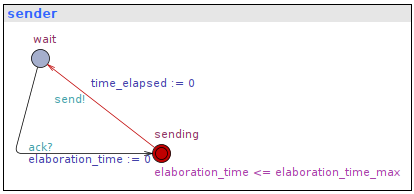
\includegraphics[width=0.8\textwidth]{1_sender.png}\end{center}
Il mittente prepara un messaggio,lo invia un e rimane in attesa di ricevere un Acknowledge, per poterlo inviare si sincronizza sul \channel send (tramite \texttt{send!}) e per riceverlo si sincronizza sul \channel ack (tramite \texttt{ack?}).
Quando un messaggio viene invato viene avviato un timer, \textit{time\_elapsed}, che sarà utile in fase di analisi per stabilire quanto tempo è passato dall'invio del messaggio alla ricezione dell'ack.
\subsection{Destinatario}
\begin{center}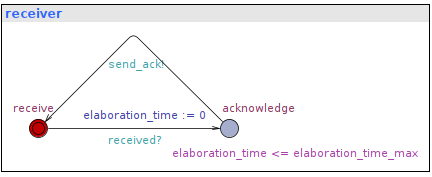
\includegraphics[width=0.8\textwidth]{1_receiver.png}\end{center}
Il destinatario può solo attendere la sincronizzazione sul \channel received, quando il canale gli fornisce un messaggio il Destinatario risponde con un Acknowledge che viene inviato sul canale sincronizzandosi sul \channel send\_ack.
\subsection{Canale}
Il canale è half-duplex, quindi permette la trasmissione non simultanea sia da mittente a destinatario che viceversa.
Il canale è "rumoroso", cioè un \textit{\pacchetto}può venir perso, sia questi un messaggio o un ack. Quindi il canale può passare dallo stato che rappresenta la presa in carico allo stato ready senza effettivamente consegnare il \pacchetto.\\
\begin{center}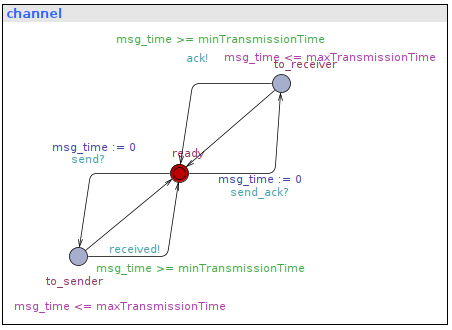
\includegraphics[width=1\textwidth]{channel_unsafe.png}\end{center}
Il canale quando non sta trasmettendo un messaggio si trova nello stato \textit{ready}, se il messaggio proviene dal mittente il canale si sincronizza sul \channel send e si sposta nello stato \texttt{to\_sender}, da questo stato esce solo dopo \textit{minTransmissionTime} e prima di \textit{maxTransmissionTime}, per rappresentare il tempo di trasmissione varibile del canale.
Per consegnare il messaggio si sincronizza con il Destinatario sul \channel received.\\
discorso diametralmente opposto vare per l'Acknowledge, il canale si sincroniza con il Destinatario sul \channel send\_ack, e consegna l'ack dopo un intervallo di tempo sincronizzandosi con il Mittente sul \channel ack.
É poi presente un timer che viene resettato sull'arco di "presa in carico" di un \pacchetto, questo timer può esssere utilizzato per verificare il tempo necessario alla trasmissione di un singolo \pacchetto.
In ultimo sono presenti due archi che vanno dagli stati di presa in carico (\textit{to\_sender} e \textit{to\_receiver}) allo stato \textit{ready} senza sincronizzarsi con il Mittente o con il Destinatario, quindi di fatto senza consegnare il \pacchetto.

\subsection{Analisi}
\begin{itemize}
	\item \textit{A[] not deadlock}
		Il sistema presenta diversi stati di deadlock. Tutte le tracce in cui un \pacchetto viene smarrito, la traccia che porta più rapidamente al deadlock è la seguente:
		$$ sender.prepare \rightarrow sender.sending \rightarrow channel.to\_send \rightarrow channel.ready $$
		In questa situazione il sistema non può più evolvere dato che il Mittente attende il canale per sincronizzarsi su \channel ack ma il mittente non ci arriverà mai dato che è bloccato dal mittente che sta aspettando la sincronizzazione sul \channel received.
	\item \textit{A[] sender.prepare imply ((time\_elapsed >= 2 * minTransmissionTime \&\& time\_elapsed <= 2 * maxTransmissionTime) || time\_elapsed == 0)}
		Questa condizione non è più verificata in quanto esistono degli stati di deadlock in qui $time\_elapsed \in (2 * maxTransmissionTime, \infty)$.\\
		Attenzione che la negazione della proposizione non è comunque vera, in quanto esistono delle tracce per cui i messaggi vengono consegnati correttamente e l'ack raggiunge il Mittente, il tutto rispettando l'intervallo di tempo.
	\item \textit{sender.sending --> sender.prepare}
		Questa condizione non è verificata in quanto potrei perdere il messaggio o l'ack.
	\item \textit{sender.sending --> receiver.acknowledge}
		Questa condizione non è verificata in quanto se invio un messaggio non è detto che il Destinatario lo riceva.
	\item \textit{channel.to\_sender --> channel.to\_receiver}
		Questa condizione non è verificata in quanto in questo sistema quando il canale prende in carico un messaggio non c'è garanzia che lo consegni al Destinatario
	\item \textit{channel.ready --> (channel.ready \&\& msg\_time >= minTransmissionTime \&\& msg\_time <= maxTransmissionTime)}
		Similmenta al caso presentato in precedenza questa condizione non è verificata poichè in caso di deadlock il timer \textit{msg\_time} supera il limite massimo di trasmissione, come nel caso tutte le tracce che non vanno in deadlock rendono vera la proposizione.
\end{itemize}


\section{Modello c}
Stop and wait con ritrasmissione e canale rumoroso.\\
In questo modello sia il messaggio che il realtivo Acknowledge possono essere smarriti, ma il protocollo è stato modificato in modo da ritrasmettere il messaggio in caso un ack non venga ricevuto entro un dato tempo limite, evento chiamato \textit{timeout}.
Il tempo di trasmissione sul link è variabile all’interno di un intervallo limitato (costanti minTransmissionTime e maxTransmissionTime ), con una differenza $\leq \frac{1}{10}$ tempo di trasmissione.

Si definiscano e provino le proprietà di corretto funzionamento del protocollo, in particolare si provi qual è il tempo minimo e massimo che intercorre dalla spedizione di un messaggio alla ricezione del suo ack .
\subsection{Mittente}
\begin{center}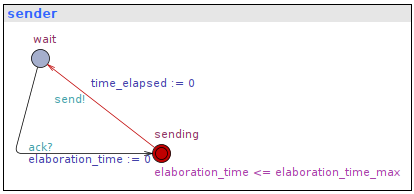
\includegraphics[width=0.8\textwidth]{1_sender.png}\end{center}
Il mittente prepara un messaggio,lo invia un e rimane in attesa di ricevere un Acknowledge, per poterlo inviare si sincronizza sul \channel send (tramite \texttt{send!}) e per riceverlo si sincronizza sul \channel ack (tramite \texttt{ack?}).
Quando un messaggio viene invato viene avviato un timer, \textit{time\_elapsed}, che sarà utile in fase di analisi per stabilire quanto tempo è passato dall'invio del messaggio alla ricezione dell'ack.
\subsection{Destinatario} 
\begin{center}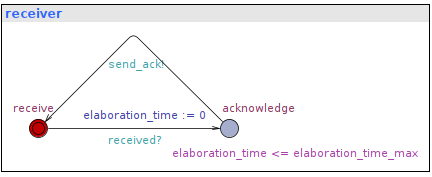
\includegraphics[width=0.8\textwidth]{1_receiver.png}\end{center}
Il destinatario può solo attendere la sincronizzazione sul \channel received, quando il canale gli fornisce un messaggio il Destinatario risponde con un Acknowledge che viene inviato sul canale sincronizzandosi sul \channel send\_ack.
\subsection{Canale}
Il canale è half-duplex, quindi permette la trasmissione non simultanea sia da mittente a destinatario che viceversa.
Il canale è "rumoroso", cioè un \textit{\pacchetto}può venir perso, sia questi un messaggio o un ack. Quindi il canale può passare dallo stato che rappresenta la presa in carico allo stato ready senza effettivamente consegnare il \pacchetto.\\
\begin{center}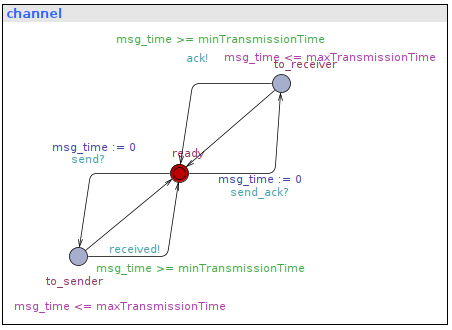
\includegraphics[width=1\textwidth]{channel_unsafe.png}\end{center}
Il canale quando non sta trasmettendo un messaggio si trova nello stato \textit{ready}, se il messaggio proviene dal mittente il canale si sincronizza sul \channel send e si sposta nello stato \texttt{to\_sender}, da questo stato esce solo dopo \textit{minTransmissionTime} e prima di \textit{maxTransmissionTime}, per rappresentare il tempo di trasmissione varibile del canale.
Per consegnare il messaggio si sincronizza con il Destinatario sul \channel received.\\
Discorso diametralmente opposto vare per l'Acknowledge, il canale si sincroniza con il Destinatario sul \channel send\_ack, e consegna l'ack dopo un intervallo di tempo sincronizzandosi con il Mittente sul \channel ack.
É poi presente un timer che viene resettato sull'arco di "presa in carico" di un \pacchetto, questo timer può esssere utilizzato per verificare il tempo necessario alla trasmissione di un singolo \pacchetto.
In ultimo sono presenti due archi che vanno dagli stati di presa in carico (\textit{to\_sender} e \textit{to\_receiver}) allo stato \textit{ready} senza sincronizzarsi con il Mittente o con il Destinatario, quindi di fatto senza consegnare il \pacchetto.

\subsection{Analisi}
\begin{itemize}
        \item \textit{A[] not deadlock}
                Il sistema presenta diversi stati di deadlock. Tutte le tracce in cui un \pacchetto viene smarrito, la traccia che porta più rapidamente al deadlock è la seguente:
                $$ sender.prepare \rightarrow sender.sending \rightarrow channel.to\_send \rightarrow channel.ready $$ 
                In questa situazione il sistema non può più evolvere dato che il Mittente attende il canale per sincronizzarsi su \channel ack ma il mittente non ci arriverà mai dato che è bloccato dal mittente che sta aspettando la sincronizzazione sul \channel received.
        \item \textit{A[] sender.prepare imply ((time\_elapsed >= 2 * minTransmissionTime \&\& time\_elapsed <= 2 * maxTransmissionTime) || time\_elapsed == 0)}
                Questa condizione non è più verificata in quanto esistono degli stati di deadlock in qui $time\_elapsed \in (2 * maxTransmissionTime, \infty)$.\\
                Attenzione che la negazione della proposizione non è comunque vera, in quanto esistono delle tracce per cui i messaggi vengono consegnati correttamente e l'ack raggiunge il Mittente, il tutto rispettando l'intervallo di tempo.
        \item \textit{sender.sending --> sender.prepare}
                Questa condizione non è verificata in quanto potrei perdere il messaggio o l'ack.
        \item \textit{sender.sending --> receiver.acknowledge}
                Questa condizione non è verificata in quanto se invio un messaggio non è detto che il Destinatario lo riceva.
        \item \textit{channel.to\_sender --> channel.to\_receiver}
                Questa condizione non è verificata in quanto in questo sistema quando il canale prende in carico un messaggio non c'è garanzia che lo consegni al Destinatario
        \item \textit{channel.ready --> (channel.ready \&\& msg\_time >= minTransmissionTime \&\& msg\_time <= maxTransmissionTime)}
                Similmenta al caso presentato in precedenza questa condizione non è verificata poichè in caso di deadlock il timer \textit{msg\_time} supera il limite massimo di trasmissione, come nel caso tutte le tracce che non vanno in deadlock rendono vera la proposizione. 
\end{itemize}

%controllare anche di non poter spedire il frame 1 senza aver spedito il frame 0
\end{document}
